\documentclass[a4paper,12pt,twoside,hidelinks,openright]{report}

\usepackage[spanish]{babel}
\usepackage[utf8]{inputenc}
\usepackage[usenames, dvipsnames]{color}
\usepackage{graphicx}
\usepackage{float}
\usepackage{enumerate}
\usepackage{multirow}
\usepackage{graphics}
\usepackage{appendix}
\usepackage[nottoc,numbib]{tocbibind}

\usepackage{tikz}
\usetikzlibrary{shapes,arrows}
\usepackage{subcaption}
\usepackage{amsmath,amsthm,amssymb,mathrsfs} 
\usepackage[final]{pdfpages}
\usepackage[]{placeins,flafter}
\usepackage[none]{hyphenat} \sloppy
\usepackage{xcolor}
\usepackage{adjustbox}

%	CONFIGURACIÓN DE PÁGINA

\setlength{\paperwidth}{21cm}          % Ancho de página
\setlength{\paperheight}{29,7cm}       % Alto de página
\setlength{\textwidth}{15.5cm}         % Ancho de zona con texto
\setlength{\textheight}{24.6cm}        % Ancho de zona con texto
\setlength{\topmargin}{-1.0cm}         % Margen superior
                                      
\setlength{\oddsidemargin}{0.46cm}     % Margen izquierdo 
\setlength{\evensidemargin}{0.46cm}    

\usepackage{makeidx}
\makeindex
\index{key}
\newcommand{\myref}[1]{\color{red}\bf(\ref{#1})}

\begin{document}

%%%%%%%%%%%%%%%%%%%%%%%%%%%%%%%%%%%%%%%%%%%%%%%%%%%%%%%%%%%%%%%%%%%%%%%%%%%%%%%%%%
%		PORTADA
%%%%%%%%%%%%%%%%%%%%%%%%%%%%%%%%%%%%%%%%%%%%%%%%%%%%%%%%%%%%%%%%%%%%%%%%%%%%%%%%%%

\begin{titlepage}

\vspace*{-4mm}
\begin{figure}[!h]
  \centering
	
\includegraphics[width=69.62mm]{Imagenes/UnizarLogo}
\end{figure}

\vspace*{17mm}

\fontsize{28pt}{28pt}\selectfont
\begin{center}
\setlength{\fboxsep}{3.4mm}
\adjustbox{minipage=14.4cm,cfbox=blue,center}{\begin{center} Trabajo Fin de Grado \end{center}}
\end{center}

\vspace*{18.7mm}


\fontsize{20pt}{20pt}\selectfont
\begin{center}
Monitorización web en tiempo real de alertas en entornos hospitalarios
\end{center}
\baselineskip 20pt
\begin{center}
Real-time web monitoring for alerts in hospital environments
\end{center}

\vspace*{1cm} 
\baselineskip 36pt
\begin{center}
\fontsize{12pt}{12pt}\selectfont
\center{\rm  Autor}

\vspace*{3.65mm} 
\fontsize{18pt}{18pt}\selectfont
\center{Leticia Sánchez Romero}
\vspace*{1cm}
\baselineskip 36pt
\fontsize{12pt}{12pt}\selectfont
\center{\rm  Director}
\vspace*{3.56mm}
\fontsize{14pt}{14pt}\selectfont
\center{Carlos Aisa Redondo}
\vspace*{1cm}
\fontsize{12pt}{12pt}\selectfont
\center{\rm  Ponente}
\vspace*{3.56mm}
\fontsize{14pt}{14pt}\selectfont
\center{Francisco Javier Zarazaga Soria}
\end{center}

\setcounter{footnote}{1}

\vspace*{16.45mm}
\fontsize{12pt}{12pt}\selectfont
\begin{center}
Grado en Ingeniería Informática\\
Departamento de Informática e Ingeniería de Sistemas\\
Escuela de Ingeniería y Arquitectura\\
\vspace*{3.56mm}
Junio 2023\\
\end{center}


\renewcommand{\thefootnote}{\arabic{footnote}}
\pagenumbering{gobble}
\end{titlepage}
\newpage


\title{Monitorización web en tiempo real de alertas en entornos hospitalarios}
\author{Leticia Sánchez Romero}

\pagebreak
\cleardoublepage
\baselineskip 19pt

\renewcommand{\labelitemi}{$-$}
\renewcommand{\tablename}{Tabla}

\renewcommand{\appendixname}{Anexos}
\renewcommand{\appendixtocname}{Anexos}
\renewcommand{\appendixpagename}{Anexos}


\pagenumbering{Roman}

%%%%%%%%%%%%%%%%%%%%%%%%%%%%%%%%%%%%%%%%%%%%%%%%%%%%%%%%%%%%%%%%%%%%%%%%%%%%%%%%%%%
%		Declaración de autoría y originalidad
%%%%%%%%%%%%%%%%%%%%%%%%%%%%%%%%%%%%%%%%%%%%%%%%%%%%%%%%%%%%%%%%%%%%%%%%%%%%%%%%%%%


\includepdf[pagecommand={}]{Impreso}
\cleardoublepage


%%%%%%%%%%%%%%%%%%%%%%%%%%%%%%%%%%%%%%%%%%%%%%%%%%%%%%%%%%%%%%%%%%%%%%%%%%%%%%%%%%%
%		Resumen
%%%%%%%%%%%%%%%%%%%%%%%%%%%%%%%%%%%%%%%%%%%%%%%%%%%%%%%%%%%%%%%%%%%%%%%%%%%%%%%%%%%

\newpage

\begin{center}
{\Large \bfseries AGRADECIMIENTOS}
\vspace{2.5cm}
\end{center}


Agradezco a
Lorem ipsum dolor sit amet, consectetuer adipiscing elit. Aenean commodo ligula eget dolor. Aenean massa. Cum sociis natoque penatibus et magnis dis parturient montes, nascetur ridiculus mus. Donec quam felis, ultricies nec, pellentesque eu, pretium quis, sem. Nulla consequat massa quis enim. Donec pede justo, fringilla vel, aliquet nec, vulputate eget, arcu. In enim justo, rhoncus ut, imperdiet a, venenatis vitae, justo. Nullam dictum felis eu pede mollis pretium. Integer tincidunt. Cras dapibus. Vivamus elementum semper nisi. Aenean vulputate eleifend tellus. Aenean leo ligula, porttitor eu, consequat vitae, eleifend ac, enim. Aliquam lorem ante, dapibus in, viverra quis, feugiat a, tellus. Phasellus viverra nulla ut metus varius laoreet. Quisque rutrum. Aenean imperdiet. Etiam ultricies nisi vel augue. Curabitur ullamcorper ultricies nisi. Nam eget dui. Etiam rhoncus. Maecenas tempus, tellus eget condimentum rhoncus, sem quam semper libero, sit amet adipiscing sem neque sed ipsum. Nam quam nunc, blandit vel, luctus pulvinar, hendrerit id, lorem. Maecenas nec odio et ante tincidunt tempus. Donec vitae sapien ut libero venenatis faucibus. Nullam quis ante. Etiam sit amet orci eget eros faucibus tincidunt. Duis leo. Sed fringilla mauris sit amet nibh. Donec sodales sagittis magna. Sed consequat, leo eget bibendum sodales, augue velit cursus nunc,

y especialmente a los alumnos que hacen plantillas de LaTeX.
\newpage
\cleardoublepage
\begin{center}
{\Large \bfseries Monitorización web en tiempo real de alertas en entornos hospitalarios}

\vspace{1cm}
{\Large \bfseries RESUMEN}

% \vspace{2.5cm}
\end{center}


Ibernex es una compañía especializada en el diseño, desarrollo e integración de soluciones y servicios tecnológicos destinados al sector socio-sanitario.
Realizan soluciones para automatizar y digitalizar la atención y experiencia de residencias u hospitales. \newline

Actualmente la compañía tiene desarrollada una aplicación que se encarga de la gestión al completo de distintas funcionalidades dentro del sector comentado anteriormente. Esta aplicación se conecta con otras aplicaciones según las necesidades que tienen los distintos clientes de Ibernex. \newline

Las soluciones que se han desarrollado hasta el momento son soluciones orientadas a aplicaciones de escritorio. Sin embargo, la empresa considera necesario que una buena opción sea utilizar alguna de sus funcionalidades en una aplicación web de tal manera que por ejemplo se pueda tener dicha aplicación ejectuando en monitores en una residencia u hospital. \newline

Por esta razón, en este proyecto se desarrolla, cómo método de prueba de cara a que la empresa pueda reutilizar la implementación que consiedere necesaria, la funcionalidad de monitorizar alertas en tiempo real.


\newpage

\cleardoublepage
\renewcommand{\contentsname}{Índice}
\tableofcontents

%%%%%%%%%%%%%%%%%%%%%%%%%%%%%%%%%%%%%%%%%%%%%%%%%%%%%%%%%%%%%%%%%%%%%%%%%%%%%%%%%%%
%		Capitulos
%%%%%%%%%%%%%%%%%%%%%%%%%%%%%%%%%%%%%%%%%%%%%%%%%%%%%%%%%%%%%%%%%%%%%%%%%%%%%%%%%%%

% \chapter{Introducción y objetivos}
\pagenumbering{arabic}
Y, viéndole don Quijote de aquella manera, con muestras de tanta tristeza, le dijo: Sábete, Sancho, que no es un hombre más que otro si no hace más que otro. Todas estas borrascas que nos suceden son señales de que presto ha de serenar el tiempo y han de sucedernos bien las cosas; porque no es posible que el mal ni el bien sean durables, y de aquí se sigue que, habiendo durado mucho el mal, el bien está ya cerca. Así que, no debes congojarte por las desgracias que a mí me suceden, pues a ti no te cabe parte dellas.Y, viéndole don Quijote de aquella manera, con muestras de tanta tristeza, le dijo: Sábete, Sancho, que no es un hombre más que otro si no hace más que otro. Todas estas borrascas que nos suceden son señales de que presto ha de serenar el tiempo y han de sucedernos bien las cosas; porque no es posible que el mal ni el bien sean durables, y de aquí se sigue que, habiendo durado mucho el mal, el bien está ya cerca. Así que, no debes congojarte por las desgracias que a mí me suceden, pues a ti no
\chapter{Introducción}
\label{ch:no_lineal}

En este capítulo se presenta el contexto del trabajo, así como la motivación del problema concreto que se aborda. Se explica los objetivos y sus limitaciones, además de las herramientas de trabajo utilizadas. Por último, se explica el esquema general de la memoria del proyecto.

\section{Contexto de trabajo}

Explicar en qué trabaja la empresa, cómo trabaja, etc.

Explicar lo que se quiere implementar, primera pincelada

\begin{figure}[!h]
    \centering
    
\includegraphics[width=0.8\textwidth,height=6cm]{Imagenes/Arte_abstracto}
    \caption{Un pie de foto}
    \label{fig:una_etiqueta}
\end{figure}


\section{Objetivos y limitaciones}

Explicar concretamente lo que se está implementando tanto en backend como en frontend. 

Explicar limitaciones como que en este caso la aplicación estará muy orientada a solo la funcionalidad que se pide pero que es así porque es un trabajo muy acotado ya que es una prueba para la empresa.

\section{Herramientas de trabajo}

Explicar las tecnoloías que estoy utilizando para cada una de las partes, y las librerías utilizadas.

\section{Esquema general de la memoria del proyecto}

Exponer las secciones que pertenecen a la memoria del proyecto para hacer una presentación de lo que se explica en cada una de ellas y no solo con el índice y los títulos.









\chapter{Análisis y diseño del sistema}

En este capítulo se expone el análisis de requisitos funcionales, la arquitectura software, la base de datos y la interfaz del usuario.

\section{Requisitos del sistema}
\label{section-requisitos}

Seguidamente (véase tabla \ref{tab:RF}) se presentan, en modo de tabla, los principales requisitos del sistema. Para su formulación se ha partido de los detalles incluidos en la sección 1.2 y se ha trabajado directamente con la empresa.

% Tabla con los requisitos del sistema

% \begin{table}[!h]
% \centering
% \begin{tabular}{|p{1cm}|p{14cm}|}
\begin{longtable}{|p{1cm}|p{14cm}|}
	\hline
	\textbf{ID} & \textbf{Requisito} \\
	\hline
	RF-1 	& 	Un usuario iniciará sesión en el sistema utilizando un identificador de usuario (nickname), contraseña y puesto. \\
	\hline
	RF-2	&	Un usuario verá como opciones del campo puesto en la autenticación, las existentes en los recursos de ese tipo de la base de datos. En caso de que no exista ningún recurso de ese tipo, verá la opción "Puesto único".	\\
	\hline
	RF-3	&	Un usuario podrá cerrar su sesión.	\\
	\hline
	RF-4	&	El sistema permitirá al usuario navegar en la aplicación mediante un menú lateral. \\
	\hline
	RF-5	&	El sistema mostrará al usuario un listado de plantas del edificio. \\
	\hline
	RF-6	&	El sistema mostrará alertas de dos tipos al usuario: alarmas y presencias activas. \\
	\hline
	RF-7	&	Las alarmas son generadas por los pacientes en una situación de emergencia desde un terminal. Son de uno de los tipos que se encuentran en la base de datos. Se muestran si se encuentran en cualquiera de los tres estados explicados en la \hyperref[section-objetivos]{sección 1.2}. Los colores de estas alarmas según su estado son: rojo si está disparada; amarilla si está aceptada; y azul si está atendida. \\
	\hline
	RF-8	&	Las presencias activas son presencias de un trabajador en una habitación y pueden ser los dos tipos explicados en la \hyperref[section-objetivos]{sección 1.2}. \\
	\hline
	RF-9	&	El sistema mostrará al usuario el número total de alarmas y presencias activas en cada planta. \\
	\hline
	RF-10	&	El sistema permitirá al usuario elegir una planta y ver la información de las alertas correspondiente a esa planta. \\
	\hline
	RF-11	&	El sistema mostrará al usuario un carrusel (presentación de tarjetas que se pueden recorrer de izquierda a derecha) con las alertas de la planta seleccionada. Las alertas más actuales aparecerán en las primeras posiciones (izquierda). \\
	\hline
	RF-12	&	El sistema mostrará al usuario la información del paciente de las alarmas activas y el lugar y momento en el que se han disparado. \\
	\hline
	RF-13	&	El sistema mostrará al usuario la información del trabajador de las presencias activas identificadas y el lugar y momento en el que se han producido. \\
	\hline
	RF-14	&	El sistema mostrará al usuario el plano (imagen guardada en la base de datos) de la planta seleccionada.  \\
	\hline
	RF-15	&	El sistema destacará al usuario en el plano las alertas activas en cada habitación coloreando la habitación según el tipo de alerta, y en caso de ser alarma también su estado, siguiendo la siguiente prioridad:
	\begin{enumerate}
		\item Rojo: alerta de tipo alarma y estado disparada
		\item Amarillo: alerta de tipo alarma y estado aceptada
		\item Azul: alerta de tipo alarma y estado atendida
		\item Verde: alerta de tipo presencia
	\end{enumerate}\\
	\hline
	RF-16	&	El sistema mostrará al usuario el listado de alarmas pendientes, sin filtrado por planta, indicando el tipo de alarma. \\
	\hline
	RF-17	&	El sistema mostrará al usuario el número total de alarmas y presencias. \\
	\hline
\caption{Requisitos funcionales del sistema}
\label{tab:RF}
\end{longtable}
	% \end{tabular}
% \end{table}

Los requisitos no funcionales definen los atributos de calidad del sistema describiendo de qué manera opera el sistema. Se presentan a coninuación (véase tabla \ref{tab:RNF}).

\begin{longtable}{|p{1,2cm}|p{13,8cm}|}
	\hline
	\textbf{ID} & \textbf{Requisito} \\
	\hline
	RNF-1 	& 	Será necesario disponer de conexión a la LAN en la que esté instalada el sistema. \\
	\hline
	RNF-2	&	El sistema estará disponible siempre y cuando el PAServidor y los servicios implicados estén activos. (Veáse la explicación de la arquitectura en la \hyperref[section-arquitectura]{sección 2.2}).	\\
	\hline
	RNF-3	&	El sistema será escalable y elástico para adaptarse a los diferentes tamaños de edificios, y por tanto al número de alertas activas, según la institución en la que se instale el sistema.\\
	\hline
	RNF-4	&	La conexión se realizará mediante websockets.\\
	\hline
	RNF-5	&	El sistema está disponible para todos los navegadores más populares en sus versiones actualizadas.\\
	\hline
	RNF-6	&	El sistema está disponible para todos los navegadores más populares en sus versiones actualizadas.\\
	\hline
	RNF-7	&	Las contraseñas utilizadas en la autenticación se comparan con el PIN identificativo del trabajador en la base de datos. \\
	\hline
\caption{Requisitos no funcionales del sistema}
\label{tab:RNF}
\end{longtable}

\section{Arquitectura software del sistema}
\label{section-arquitectura}
% Explicar la arquitectura final del sistema

El despliegue del sistema se realizará en una red de área local (LAN) ya que tiene que servir para una residencia u hospital en el que se instalará el sistema configurando la base de datos correspondiente a la información de la institución.\\

Para ver las relaciones entre el software y su entorno se utiliza una vista de distribución estilo despliegue. Se puede ver en la \textit{Figura 2.1}. \\

\begin{figure}[!h]
    \centering
    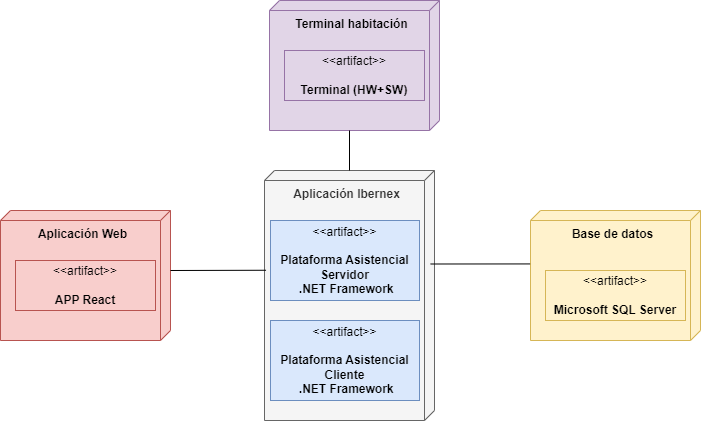
\includegraphics[width=1\textwidth,height=10cm]{Imagenes/Arquitectura-despliegue}
    \caption{Diagrama de despliegue}
    \label{fig:despliegue}
\end{figure}

Con este diagrama se observan los elementos que han estado implicados en el proyecto. No obstante, lo que se ha implementado ha sido: la aplicación web completa y la funcionalidad añadida a la Plataforma Asistencial Servidor de la aplicación de Ibernex. A continuación se describen los elementos con mayor detalle:

\begin{itemize}
	\item \textbf{Plataforma Asistencial Servidor (PAServidor)} es la aplicación servidor del sistema asistencial Helpnex. Se trata de una aplicación monolítica modular. Dos de los elementos que componen la arquitectura de la aplicación son:
	\begin{itemize}
		\item Servicios: contienen la lógica del sistema Helpnex. Los servicios se cargan al inicio de la aplicación en función de la licencia adquirida. Cada servicio es el encargado de realizar una tarea específica. Algunos ejemplos de tareas son: comunicación con los terminales de habitación; gestionar las alarmas del sistema; comunicación con la aplicación web de monitorización; localización en interiores; comunicaciones SIP; entre otras.
		\item Cola de eventos: es el mecanismo de comunicación que utilizan los servicios para transmitir información entre ellos. Cada servicio se suscribe a una serie de eventos.
	\end{itemize}
	\item La \textbf{base de datos} es la que permite realizar la persistencia de datos de PAServidor, PACliente, la institución, los pacientes y resto de datos necesarios.
	\item La \textbf{aplicación web} que recibe los datos necesarios a monitorizar para mostrarlos.
	\item \textbf{Plataforma Asistencial Cliente (PACliente)} se comunica con el PAServidor mediante una conexión socket TCP y es la encargada de gestionar la información del sistema Helpnex y guardarla en la Base de Datos. Esta información se utiliza por PAServidor para realizar las gestiones necesarias. De igual forma, se compone de módulos que se gestionan mediante una licencia y permiten gestionar distintos elementos. Uno de los módulos sirve para configurar un sistema de reglas de notificación ante una alarma y esto es lo que permite al sistema generar las reglas y notificar por puestos la información que debe ser mostrada en la aplicación web.\\
	PACliente se ha utilizado en el proyecto  para realizar la gestión de plantas, habitaciones, residentes, terminales, trabajadadores, recursos de los puestos y configuración de reglas teniendo una institución ficticia generada con datos de prueba durante todo el desarrollo.
	\item El \textbf{terminal} es el hardware que se encuentra en la habitación. En este contexto sirve tanto para notificar y codificar las alarmas como para registrar las presencias de trabajadores en las habitaciones.
\end{itemize}

Para entender mejor la arquitectura del PAServidor se proporciona un diagrama más detallado en la \textit{Figura 2.2}.

\begin{figure}[H]
    \centering
    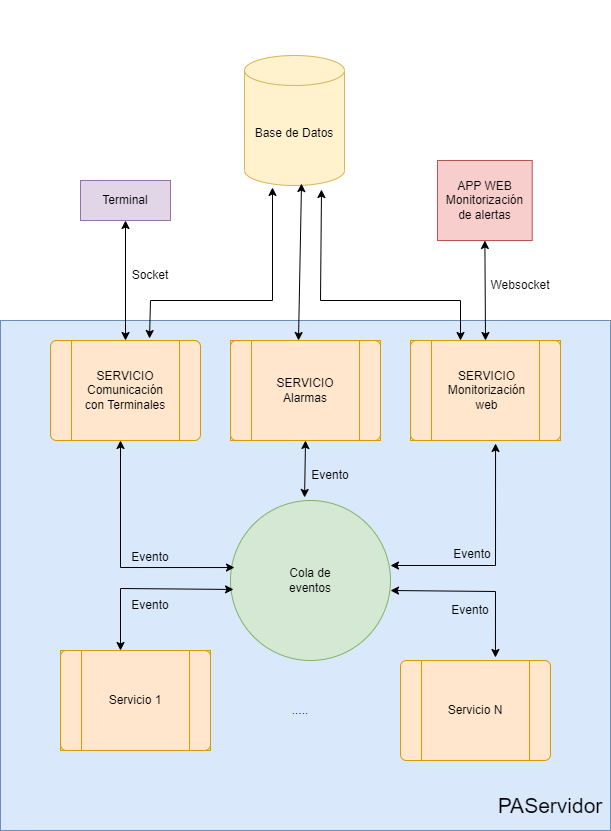
\includegraphics[width=1\textwidth,height=17cm]{Imagenes/Arquitectura-PAServidor}
    \caption{Diagrama arquitectura PAServidor}
    \label{fig:PAServidor}
\end{figure}


% Hacer referencia al Anexo donde se expliquen las alternativas que se plantearon
La arquitectura aquí expuesta es la elegida entre las distintas opciones barajadas. Estas otras se pueden consultar con detalle en el \hyperref[anexo-a]{Anexo A}.


\section{Base de datos}

% Explicar qué partes de la base de datos utilizo de su sistema y con diagramas

TODO: explicar qué tablas de la base de datos utilizo de su sistema y adjuntaré  diagramas creados con la aplicación Microsoft SQL Server Management. \\

% INCLUIR EN EL ESQUEMA DEL LOGIN LA TABLA DE LOS RECURSOS DONDE ESTARÁN LOS PUESTOS

% REVISAR EL RESTO DE DIAGRAMAS PARA QUE REALMENTE ESTÉ TODO LO QUE SE HA UTILIZADO

\section{Interfaz de usuario}

% Poner la interfaz final del usuario cuando esté terminada

TODO: Poner la interfaz final del usuario cuando esté terminada


\chapter{Implementación}

% TODO: Explicar concretamente lo que se está implementando tanto en backend como en frontend. 

\section{Implementación del frontend}

El frontend de la aplicación web se realiza con React utilizando los lenguajes de programación \textit{javascript}, \textit{HTML}, y \textit{CSS}.\\

Para la comunicación del frontend con el backend mediante WebSockets se utiliza la librería \textit{reconnecting-websocket} \cite{reconect-ws}. Se decide utilizar esta frente a otras porque reconecta automáticamente con el servicio si la conexión se cierra por alguna razón y es compatible con \textit{WebSocket Browser API} \cite{api-ws-front}. \\


% TODO: explicar que se recibe directamente la información a mostrar, qué es lo que se trata o no (por ejemplo el ordenar por actual que se realiza en el frontend, el filtrado por plantas, el procesado para el mapeado por habitaciones y prioridad).
La aplicación web es una aplicación visual, en la que no se puede realizar ninguna acción sobre las alertas. Se recibe por websockets toda la información necesaria a monitorizar que procesa el nuevo servicio implementado en PAServidor. Por esta razón, la mayoría de la implementación de esta parte del proyecto se centra en interfaz de usuario aunque también se realiza el tratado de la información que llega para tener los datos de la manera indicada. Cabe destacar que el filtrado por plantas de las alertas, la ordenación de las alertas por más actuales, el filtrado de alertas por prioridad y el mapeado por habitaciones, se realiza en esta parte del proyecto.\\


% Indicar otras librerías utilizadas en el proyecto
Para implementar la aplicación web se ha considerado útil contar con el apoyo de ciertas librerías. Algunas interesantes de mencionar son:
\begin{itemize}
	\item \textit{Bootstrap} \cite{bootstrap} y \textit{React-Bootstrap} \cite{react-bootstrap} como herramientas para la implementación de la interfaz de usuario.
	\item \textit{react-multi-carousel} \cite{react-multi-carousel} para mostrar el carrusel de alertas en una de las pantallas principales de la aplicación.
	\item \textit{react-icons} \cite{react-icons} ya que provee distintos tipos de iconos para la aplicación.
	\item \textit{react-moment} \cite{react-moment} como apoyo para utilizar las fechas y horas de las alertas y ordenarlas para mostrar en el carrusel las más actuales primero.
	\item \textit{react-img-mapper} \cite{react-img-mapper} para facilitar el mapeado de las áreas de las habitaciones en los planos de las plantas y poder mostrar al usuario las habitaciones coloreadas por prioridad junto con el icono de la alerta con más prioridad dentro de dicha habitación y la tarjeta emergente con la información de dicha alerta.
\end{itemize}

 % Explicar organización de ficheros en frontend indicando que cierta división de los módulos hace que la organización del código queda bien repartida teniendo las funcionalidades para poder ver a simple vista implementado

Durante el desarrollo de la aplicación se ha seguido cierta estructura a la hora de dividir los módulos para organizar el código. De esta forma, ha sido más fácil realizar una implementación clara durante el desarrollo. Además, de cara a que la empresa pueda reutilizar el código hace que sea más sencillo comprenderlo. Se puede ver la organización realizada  en tiempo de desarrollo con una vista de módulos en forma de diagrama de paquetes. (Véase \textit{Figura 3.1}).\\

% TODO: Diagrama de paquetes UML para explicar la organización.



\section{Implementación del backend}

El backend de la aplicación se realiza con \textit{.NET Framework 4.8}, ya que como se ha explicado en secciones anteriores la implementación es añadir funcionalidad a la aplicación existente. \\

Para la comunicación con el frontend mediante WebSockets se utiliza la librería \textit{websocket-sharp} \cite{websocket-sharp} en su versión \textit{1.0.3.0}.
Se decide utilizar esta librería ya que en otra de las funcionalidades existente en la aplicación se utiliza (aunque en una versión anterior), y se cree conveniente utilizar algo similar de cara a que internamente en la empresa puedan entender mejor la implementación o reutilizar el código.
La instalación de esta librería se realiza mediante el propio Visual Studio (que se ha comentado la sección de herramientras de trabajo que es el entorno de desarrollo utilizado para implementar el backend) utilizando la opción de administrar paquetes NuGet e instalando el nombrado. \\

Al principio la empresa propuso realizar la comunicación del backend con el frontend utilizando \textit{SignalR} \cite{signalr} pero finalmente se descarta por incompatibilidad con la aplicación actual y simplicidad en la arquitectura software. Se puede ver más información referente a esta decisión en el \hyperref[anexo-b]{Anexo B}. \\


% Explicar qué SERVICIO implemento dentro de la arquitectura
De los servicios y eventos nombrados en la arquitectura detallada del PAServidor en la \hyperref[section-arquitectura]{sección 2.2}, el servicio que se ha implementado para añadir funcionalidad a la aplicación existente y que sirve como backend de la aplicación web, es el \textit{Servicio de monitorización web} que se puede observar en la sección nombrada, concretamente en la \hyperref[fig:PAServidor]{\textit{Figura 2.2}}.\\

% Explicar comportamiento de servicios y eventos
\subsection{Comportamiento servicios y eventos}
\label{subsection-comportamiento}
% TODO: DIAGRAMAS DE COMPORTAMIENTO para mostrar ejemplo/s de funcionamiento interno.
Respecto al comportamiento de los servicios y eventos implocados, a continuación se exponen unos ejemplos de funcionamiento.\\

El funcionamiento para el caso de las alarmas es el siguiente:
\begin{enumerate}
	\item El paciente pulsa el botón del terminal para solicitar ayuda.	
	\item El terminal notifica al Servicio de Comunicación con Terminales, mediante el socket, que alguien ha pulsado el botón.
	\item El servicio comunicación con terminales envía un evento \textit{NuevaAlarma} con toda la información relativa al terminal.
	\item El servicio de alarmas, que está suscrito al evento \textit{NuevaAlarma}, recibe el evento y lo procesa. Es necesario acceder a la base de datos para obtener información necesaria. Como resultado envía un evento \textit{NotificarAlarmaEnMonitorWeb}.
	\item El servicio de monitorización web recibe el evento \textit{NotificarAlarmaEnMonitorWeb} al que está suscrito y lo procesa, envíando mediante websocket la información conveniente a la aplicación web.
	\item En la aplicación web aparecerá la nueva alarma.
	\item El Servicio de Monitorización web recibe el evento \textit{SAEvento\_NuevaAccionPendiente} cuando se producen alarmas y lo procesa si le ha llegado el evento \textit{NotificarAlarmaEnMonitorWeb} para actualizar la alarma indicada, y el resultado de la actualización es envíado mediante el websocket a la aplicación web.
	\item En la aplicación web aparecerá la alarma actualizada.
	\item El Servicio de Monitorización web recibe el evento \textit{SAEvento\_DisparoAvisoFinalizado} cuando se codifica una alarma y lo procesa si le ha llegado el evento de \textit{NotificarAlarmaEnMonitorWeb} para eliminar la alarma indicada, y el resultado de la actualización es envíado mediante el websocket a la aplicación web.
	\item En la aplicación web desaparecerá la alarma actualizada.
\end{enumerate}

El funcionamiento para el caso de las presencias es el siguiente:

\begin{enumerate}
	\item Un trabajador se identifica en la habitación pasando su tarjeta personal por el lector o con el su PIN.
	\item El terminal notifica al Servicio de Comunicación con Terminales, mediante el socket, que alguien está presente.
	\item El Servicio de Comunicación con Terminales envía un evento \textit{NuevaPresencia} con toda la información relativa a la presencia.
	\item El servicio de alarmas que está suscrito al evento \textit{NuevaPresencia} recibe el evento y lo procesa. Es necesario acceder a la Base de Datos para obtener información necesaria. Como resultado envía un evento \textit{PAEvento\_NotificarEstadoPresencias}.
	\item El servicio de monitorización web recibe el evento \textit{PAEvento\_NotificarEstadoPresencias} que puede ser de las presencias actuales, de una presencia nueva, actualizada o eliminada y lo procesa. Como resultado envía la información necesaria mediante el websocket a la aplicación web.
	\item En la aplicación web aparece, se actualiza o desaparece la presencia.
\end{enumerate}


% TODO: Mirar en mis notas todas las decisiones y controversisas con backend
TODO: Decisiones de implementación respecto a ficheros y funciones que tengo anotadas y problemas u opciones surgidas respecto a la implementación del backend\\

\chapter{Conclusiones}

\section{Conclusiones}

% Explicar lo que has hecho. Básicamente decir que lo que ibas a hacer lo has hecho

El proyecto ha finalizado con éxito cumpliendo con los objetivos descritos en la \hyperref[section-objetivos]{sección 1.2} y los requisitos expuestos en la \hyperref[section-requisitos]{sección 2.1}.\\

Se ha desarrollado un sistema de información en forma de aplicación web que monitoriza en tiempo real alertas, ya sean presencias identificadas o no, o alarmas con sus distintos estados.\\

Para esto se ha desarrollado desde cero el frontend de la aplicación; se han estudiado las distintas alternativas de arquitectura software, partiendo del esquema propuesto inicialmente por la empresa; se han analizado las opciones de comunicación para las distintas arquitecturas; y se ha implementado correctamente el backend de la aplicación añadiendo la lógica adicional necesaria en la aplicación existente. Todo esto aplicando las decisiones finales debatidas con la empresa referentes a la arquitectura del sistema y la comunicación entre el frontend y backend.
 

\section{Conocimientos adquiridos}

En esta sección se presentan los conocimientos técnicos y personales adquiridos con la realización de este proyecto.

\subsection{Conocimientos técnicos}

% Nuevas tecnologías, nuevos entornos de trabajo

En cuanto a conocimientos técnicos, se destaca que para la parte de frontend se había trabajado anteriormente con \textit{React} por lo que se tenía experiencia previa en desarrollo de aplicaciones web con dicha tecnología, además de con los lenguajes de programación utilizados para esta parte del proyecto. Aunque se ha podido trabajar aspectos que anteriormente no habían sido abordados como trabajar con el mapeado de imágenes. \\

Para el control de versiones ya se había trabajado con \textit{Git} y \textit{GitHub} anteriormente, por lo que ha sido fácil seguir trabajando con estas herramientas.\\

Por el contrario, las herramientas de la parte del backend no se habían utilizado, por lo que ha sido parte del reto de este proyecto familiarizarse con el lenguaje \textit{C\#} junto con la tecnología \textit{.NET Framework} utilizando como entorno \textit{Microsoft Visual Studio}. Esto es beneficioso ya que se añaden todos estos conocimientos de cara a tener más aptitudes para la salida al mundo laboral.\\

Además, ha sido la primera vez que se ha tenido la oportunidad de trabajar con websockets ya que anteriormente, solo se había colaborado en proyectos de desarrollo en equipo, sin asumir la responsabilidad específica de trabajar con esta tecnología. \\

De igual manera, se ha conocido \textit{SignalR}, que aunque finalmente no se haya utilizado en el proyecto, se estuvieron haciendo algunas pruebas con dicha tecnología, y para un futuro ya se tiene conocimiento de lo que es y para qué sirve.

\subsection{Conocimientos personales}

% Organización, primer trabajo en una empresa del relacionada con los estudios, y trabajo en remoto y lo que conlleva, dificultades.
En cuanto a los conocimientos personales adquiridos, en primer lugar cabe mencionar la experiencia adquirida con los conocimientos técnicos expuestos anteriormente.\\

Cabe destacar principalmente que ha sido la primera experiencia laboral realizando un proyecto software en un entorno relacionado con el grado cursado, ya que se ha realizado este Trabajo de Fin de Grado como estudiante en prácticas en Ibernex. También ha sido un reto y un aprendizaje trabajar de forma remota por estar realizando el último año del grado en Kaunas, Lituania. Gracias a esto se ha aprendido a sobrellevar y solucionar las dificultades que se han tenido, sobre todo cuando surgían inconvenientes con la conexión a la red de la empresa, o la diferencia de poder consultar algo estando en la empresa rodeada del resto del equipo de desarrollo frente a estar a distancia y depender de distinto uso horario.\\

Esta situación ha sido beneficiosa en el sentido en que que se han mejorado las habilidades de organización para lidiar con dichas dificultades, y mantener al mismo tiempo los compromisos académicos con la universidad de destino y laborales simultáneamente.


\section{Trabajo futuro}
\label{section-trabajo-futuro}
% Explicar que la aplicación desarrollada puede ser utilizada por Ibernex para reutilizar código o como prueba/base por si quieren sacar a producción trabajar con sistemas web finalmente ya que me explicaron que esto era como una pequeña prueba que querían hacer

La implementación realizada solo incluye funcionalidad para monitorizar en la web los dos tipos de alerta comentados en secciones anteriores: las presencias y las alarmas.\\

Inicialmente se incluía también la posibilidad de tener tareas como tipo de alerta, por lo que se comenzó parte de la implementación en backend para administrar la llegada de este tipo de eventos, y en frontend, el diseño de modelos e implementación del código se pensó de manera que fuera posible reutilizar o facilitar, sirviendo de base, algunos aspectos del código, como poder usar el mismo modelo de alerta con cualquier tipo.
Por esta razón una línea de trabajo futura, siguiendo el contexto del proyecto realizado, sería incluir las alertas en la aplicación web y que estas fueran igualmente monitorizadas. Para esto se tendría que continuar la implementación e incluir cierta funcionalidad tanto en backend como en frontend.\\

Se destaca que la aplicación web desarrollada sirve de base y prueba a Ibernex para ver cómo es incluir la implementación web en la empresa y ver cómo funciona en este caso la monitorización de alertas. Por lo que, la principal línea futura de trabajo para la empresa, es que gracias a este proyecto pueden analizar si les sería interesante sacar a producción y comenzar a desarrollar soluciones de su aplicación compatibles con web.

%Puedes añadir más capítulos
%%%%%%%%%%%%%%%%%%%%%%%%%%%%%%%%%%%%%%%%%%%%%%%%%%%%%%%%%%%%%%%%%%%%%%%%%%%%%%%%%%%
%		BIBLIOGRAFÍA Y REFERENCIAS
%%%%%%%%%%%%%%%%%%%%%%%%%%%%%%%%%%%%%%%%%%%%%%%%%%%%%%%%%%%%%%%%%%%%%%%%%%%%%%%%%%%

\bibliographystyle{unsrt} %plaindin
\bibliography{Bibliografia_TFG}
\nocite{*} 

\newpage
\renewcommand\listfigurename{Lista de Figuras}
\listoffigures

\newpage
\renewcommand\listtablename{Lista de Tablas}
\listoftables

%%%%%%%%%%%%%%%%%%%%%%%%%%%%%%%%%%%%%%%%%%%%%%%%%%%%%%%%%%%%%%%%%%%%%%%%%%%%%%%%%%%
%		ANEXOS
%%%%%%%%%%%%%%%%%%%%%%%%%%%%%%%%%%%%%%%%%%%%%%%%%%%%%%%%%%%%%%%%%%%%%%%%%%%%%%%%%%%

\newpage
\appendix
\clearpage
\addappheadtotoc
\appendixpage
\chapter{Alternativas arquitecturas}

% TODO: Explicar como expliqué a Javier en el correo las alternativas de las arquitecturas y los pros y contras de cada una de ellas y el por qué de la decisión











%%%%%%%%%%%%%%%%%%%%%%%%%%%%%%%%%%%%%%%%%%%%%%%%%%%%%%%%%%%%%%%%%%%%%%%%%%%%%%%%%%%


\end{document}